\chapter{Connections}

\section{Cipher suit}
A cipher suite is a set of algorithms that help secure a network connection that uses Transport Layer Security (TLS) or its now-deprecated predecessor Secure Socket Layer (SSL). The set of algorithms that cipher suites usually contain include: a key exchange algorithm, a bulk encryption algorithm, and a message authentication code (MAC) algorithm.\cite{ciphersuit-wiki}
\\
The key exchange algorithm is used to exchange a key between two devices. This key is used to encrypt and decrypt the messages being sent between two machines. The bulk encryption algorithm is used to encrypt the data being sent. The MAC algorithm provides data integrity checks to ensure that the data sent does not change in transit. In addition, cipher suites can include signatures and an authentication algorithm to help authenticate the server and or client.\cite{ciphersuit-wiki}
\\
After coordinating which cipher suite to use, the server and the client still has the ability to change the coordinated ciphers by using the ChangeCipherSpec protocol in the current handshake or in a new handshake.\cite{ciphersuit-wiki}


\subsection{TLS 1.0–1.2 handshake}

This client starts the process by sending a clientHello message to the server that includes the version of TLS being used and a list of cipher suites in the order of the client’s preference. In response, the server sends a serverHello message that includes the chosen cipher suite and the session ID. Next the server sends a digital certificate to verify its identity to the client. \textbf{The server may also request a client’s digital certification if needed}.\cite{ciphersuit-wiki}

\begin{figure}[!h]
\centering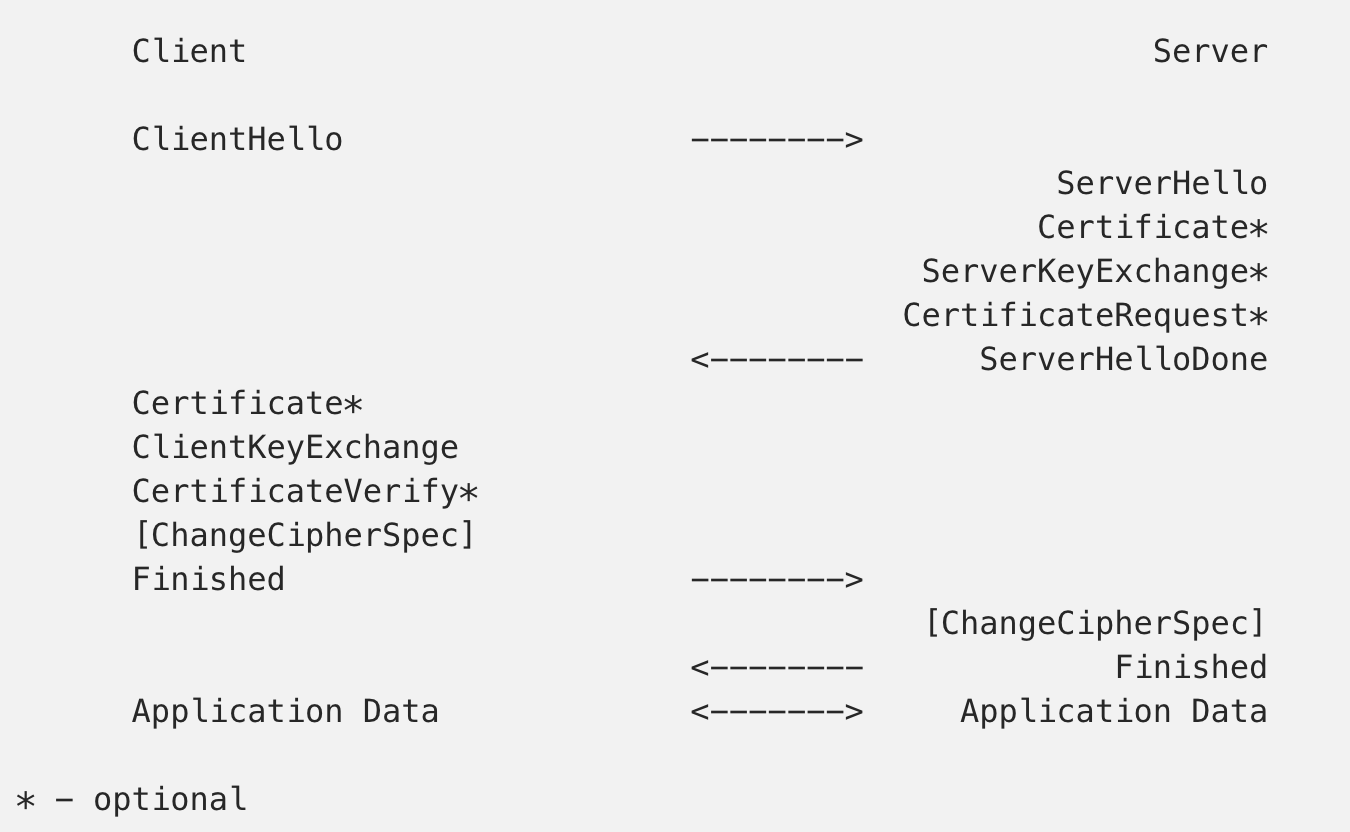
\includegraphics[scale=0.6]{TLS-Handshake}
\caption{TLS Handshake Protocol \cite{TLS-meduim}}
\label{fig:TLS_Proto} % Unique label used for referencing the figure in-text
\end{figure}


If the client and server are not using pre-shared keys, the client then sends an encrypted message to the server that enables the client and the server to be able to compute which secret key will be used during exchanges.\cite{ciphersuit-wiki}
\\
After successfully verifying the authentication of the server and, if needed, exchanging the secret key, the client sends a finished message to signal that it is done with the handshake process. After receiving this message, the server sends a finished message that confirms that the handshake is complete. Now the client and the server are in agreement on which cipher suite to use to communicate with each other.\cite{ciphersuit-wiki}


\begin{figure}[!h]
\centering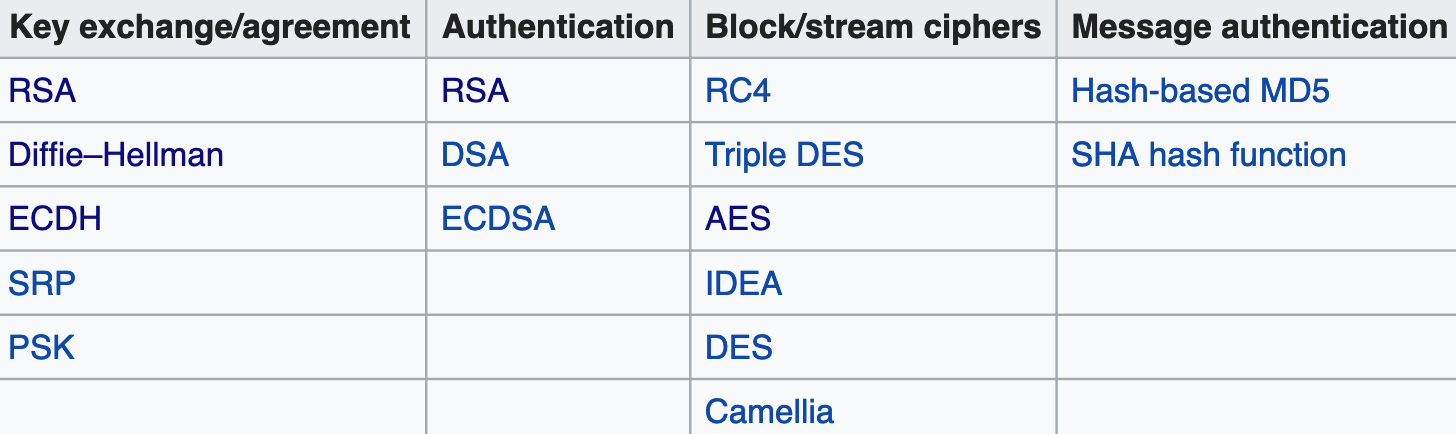
\includegraphics[scale=0.6]{TLSv1-12_algs}
\caption{Algorithms supported in TLS 1.0–1.2 cipher suites \cite{ciphersuit-wiki}}
\label{fig:TLS_algs} % Unique label used for referencing the figure in-text
\end{figure}

\section{Connections}

Connections between two Tor relays, or between a client and a relay, use TLS/SSLv3 for link authentication and encryption. All implementations MUST support the SSLv3 ciphersuite\\ "TLS\_DHE\_RSA\_WITH\_AES\_128\_CBC\_SHA" if it is available. They SHOULD support better ciphersuites if available.
\\

   There are three ways to perform TLS handshakes with a Tor server. 
   
   \begin{enumerate}
	\itemsep0.5em
   	\item \textbf{certificates-up-front}: Both the initiator and responder send a two-certificate chain as part of their initial handshake.  (This is supported in all Tor versions.)
   	\item \textbf{renegotiation}: The responder provides a single certificate, and the initiator immediately performs a TLS renegotiation. (This is supported in Tor 0.2.0.21 and later.)
   	\item \textbf{in-protocol}: the initial TLS negotiation completes, and the parties bootstrap themselves to mutual authentication via use of the Tor protocol without further TLS handshaking. (This is supported in 0.2.3.6-alpha and later.)
   \end{enumerate}
   
Each of these options provides a way for the parties to learn it is
   available: a client does not need to know the version of the Tor
   server in order to connect to it properly.
   \\
   
\label{Key:connection-key} In "certificates up-front" (a.k.a "the v1 handshake"), the connection initiator always sends a two-certificate chain, consisting of an X.509 certificate using a short-term connection public key and a second, self-signed X.509 certificate containing its identity key. The other party sends a similar certificate chain. The initiator's ClientHello MUST NOT include any ciphersuites other than:
\begin{enumerate}
	\item TLS\_DHE\_RSA\_WITH\_AES\_256\_CBC\_SHA
	\item TLS\_DHE\_RSA\_WITH\_AES\_128\_CBC\_SHA
	\item SSL\_DHE\_RSA\_WITH\_3DES\_EDE\_CBC\_SHA
\end{enumerate}

In "renegotiation" (a.k.a. "the v2 handshake"), the connection initiator sends no certificates, and the responder sends a single connection certificate.  Once the TLS handshake is complete, the initiator renegotiates the handshake, with each party sending a two-certificate chain as in "certificates up-front". The initiator's ClientHello MUST include at least one ciphersuite not in the list above -- that's how the initiator indicates that it can handle this handshake.  For other considerations on the initiator's ClientHello, see section 2.1 below.

In "in-protocol" (a.k.a. "the v3 handshake"), the initiator sends no certificates, and the responder sends a single connection certificate.  The choice of ciphersuites must be as in a "renegotiation" handshake.  There are additionally a set of constraints on the connection certificate, which the initiator can use to learn that the in-protocol handshake is in use.
\\
These are some usefull fields in the structure of an X.509 v3 
certificate according to \cite{crl_rfc}:

\begin{lstlisting}[language=c, caption={X.509 v3 Certificate structure}]
Certificate  ::=  SEQUENCE  {
        tbsCertificate       TBSCertificate,
        signatureAlgorithm   AlgorithmIdentifier,
        signatureValue       BIT STRING  }

   TBSCertificate  ::=  SEQUENCE  {
        version         [0]  EXPLICIT Version DEFAULT v1,
        serialNumber         CertificateSerialNumber,
        signature            AlgorithmIdentifier,
        issuer               Name,
        validity             Validity,
        subject              Name,
        subjectPublicKeyInfo SubjectPublicKeyInfo,
        issuerUniqueID  [1]  IMPLICIT UniqueIdentifier OPTIONAL,
                             -- If present, version MUST be v2 or v3
        subjectUniqueID [2]  IMPLICIT UniqueIdentifier OPTIONAL,
                             -- If present, version MUST be v2 or v3
        extensions      [3]  EXPLICIT Extensions OPTIONAL
                             -- If present, version MUST be v3
        }
\end{lstlisting}

\textbf{issuer}
\\
The issuer field identifies the entity that has signed and issued the certificate.  The issuer field MUST contain a non-empty distinguished name (DN).  The issuer field is defined as the X.501 type Name.
\\

Implementations of this specification MUST be prepared to receive the following standard attribute types in issuer and subject (Section 4.1.2.6 of \cite{crl_rfc} ) names:
\begin{enumerate}
	\item country
	\item organization
	\item organizational unit
	\item distinguished name qualifier (DN)
	\item state or province name
	\item common name (e.g., "Susan Housley")
	\item serial number
\end{enumerate}

Specifically, at least one of these properties must be true of the certificate:\label{inpro:criteria}
\begin{enumerate}
	\item The certificate is self-signed
	\item Some component other than "commonName" is set in the subject or issuer DN of the certificate.
	\item The commonName of the subject or issuer of the certificate ends with a suffix other than ".net".
	\item The certificate's public key modulus is longer than 1024 bits.
\end{enumerate}
  
Here is implementation of in-protocol handshake through the Tor source code:

\begin{lstlisting}[language=c, caption={\href{https://gitweb.torproject.org/tor.git/tree/src/lib/tls/tortls.c}{in-protocol implementation} line number 287 }]
int
tor_tls_context_init_certificates(tor_tls_context_t *result,
                                  crypto_pk_t *identity,
                                  unsigned key_lifetime,
                                  unsigned flags)
\end{lstlisting}
  
%    /* choose between 5 and 365 days, and round to the day */
%    unsigned int five_days = 5*24*3600;
%    unsigned int one_year = 365*24*3600;
%    lifetime = crypto_rand_int_range(five_days, one_year);
%    lifetime -= lifetime % (24*3600);

The initiator then sends a VERSIONS cell to the responder, which then replies with a VERSIONS cell; they have then negotiated a Tor protocol version.  Assuming that the version they negotiate is 3 or higher (the only ones specified for use with this handshake right now), the responder sends a CERTS cell, an AUTH\_CHALLENGE cell, and a NETINFO cell to the initiator, which may send either CERTS, AUTHENTICATE, NETINFO if it wants to authenticate, or just NETINFO if it does not.
\href{tor/src/core/or/channeltls.c}{Here} is the implementation code.
\paragraph{}
For backward compatibility between later handshakes and "certificates up-front", the ClientHello of an initiator that supports a later handshake MUST include at least one ciphersuite other than those listed above. The connection responder examines the initiator's ciphersuite list to see whether it includes any ciphers other than those included in the list above.  If extra ciphers are included, the responder proceeds as in "renegotiation" and "in-protocol": it sends a single certificate and does not request client certificates.  Otherwise (in the case that no extra ciphersuites are included in the ClientHello) the responder proceeds as in "certificates up-front": it requests client certificates, and sends a two-certificate chain.  In either case, once the responder has sent its certificate or certificates, the initiator counts them. If two certificates have been sent, it proceeds as in "certificates up-front"; otherwise, it proceeds as in "renegotiation" or "in-protocol".
\\
To decide whether to do "renegotiation" or "in-protocol", the initiator checks whether the responder's initial certificate matches the criteria listed above\ref{inpro:criteria}.

   All new relay implementations of the Tor protocol MUST support
   backwards-compatible renegotiation; clients SHOULD do this too.  If this is not possible, new client implementations MUST support both "renegotiation" and "in-protocol" and use the router's published link protocols list (\href{https://gitweb.torproject.org/torspec.git/tree/dir-spec.txt}{see dir-spec.txt on the "protocols" entry} ) to decide which to use.

\paragraph{Anonymity inside TLS}
In all of the above handshake variants, certificates sent in the clear SHOULD NOT include any strings to identify the host as a Tor relay. In the "renegotiation" and "backwards-compatible renegotiation" steps, \textbf{the initiator SHOULD choose a list of ciphersuites and TLS extensions to mimic one used by a popular web browser}. Connection protocols are identical for both OP and OR nodes. Onion proxies SHOULD NOT provide long-term-trackable identifiers in their handshakes.



